\documentclass{beamer}
\usepackage[english]{babel}
\usepackage[utf8]{inputenc}
\usepackage{times}
\usepackage[T1]{fontenc}
\usepackage{lmodern}
\usepackage{tikz}
\usepackage{minted}
\usemintedstyle{borland}
\usetikzlibrary{arrows}
\usepackage{graphicx}
\usepackage{amssymb}
\usepackage{amsthm}
\usepackage{amsmath}
\usepackage{csquotes}
\usepackage{bbm}
\newcommand{\wo}{\mathbbm{w}}
\usetheme{Warsaw}
\usepackage{array,colortbl,xcolor}


\setbeamertemplate{bibliography item}[text]
\setbeamertemplate{navigation symbols}{}



\title[Word2Vec] 
{Word2vec}


\author[F.Salvatore] 
{Felipe~Salvatore}




\date[USP 2015] 
{USP, 06/04/2017}

\begin{document}


\begin{frame}
\titlepage 
\end{frame}





\begin{frame}{Introdução}
Word2vec é um nome que abarca dois modelos:
\begin{itemize}
\item \textbf{Skip-gram}
\item \textbf{Continuous Bag-of-Words (CBOW)}
\end{itemize}

\vspace{0.1cm}
\textbf{Tarefa:} Apreender de modo eficiente uma representação vetorial de palavras a partir de um corpus grande e não-estruturado.\\

Esse aprendizado é feito atraves das estatística de co-ocorrência das palavras em algum corpus. A ideia em si não é nova:
\vspace{0.1cm}

\begin{center}
{\color{blue!89}"You shall know a word by the company it keeps" (J.R Firth, 1957)}
\end{center}
\end{frame}


\begin{frame}[fragile]{Versão simplificada de CBOW: modelo (i)}
Dado um corpus, escolhemos:
\begin{itemize}
\item um vocabulário $V$. 
\item um tamanho $N$ para a representação vetorial das palavras.
\end{itemize}
\vspace{0.1cm}
Vamos usar as matrizes $W \in \mathbb{R}^{|V|,N}$ e $W^{\prime} \in \mathbb{R}^{N,|V|}$ para criar \textbf{duas} representações vetoriais de cada palavra $\wo$:
\vspace{0.1cm}
\begin{itemize}
\item \textbf{input vector}: $v_\wo$  (linha de $W$).
\vspace{0.1cm}
\item \textbf{output vector}: $v^{\prime}_\wo$  (coluna de $W^{\prime}$).
\end{itemize}
\end{frame}

\begin{frame}[fragile]{Versão simplificada de CBOW: modelo  (ii)}
A tarefa do modelo vai ser prever uma palavra de centro dada uma palavra de contexto:

\begin{center}
{\color{red!89}O} {\color{blue!89}primeiro} {\color{red!89}rei} de Portugal nasceu em ...
\end{center}
\vspace{0.1cm}
Observação $\Rightarrow$ (rei, primeiro)\\

\vspace{0.1cm}

{\color{white!89}Observacao } $\Rightarrow$ (input word, output word)\\

\vspace{0.1cm}

{\color{white!89}Observacao } $\Rightarrow$ ($\wo_{I}$, $\wo_{o}$)
\end{frame}

\begin{frame}[fragile]{Versão simplificada de CBOW: modelo  (iii)}
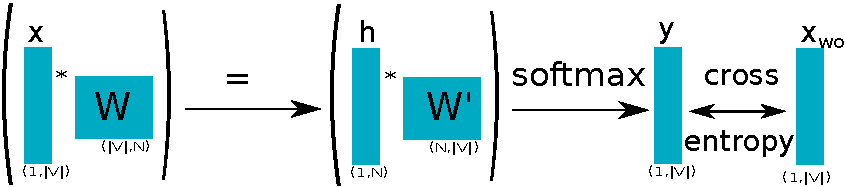
\includegraphics[scale=0.8]{simple_model.pdf}
\end{frame}

\begin{frame}[fragile]{Versão simplificada de CBOW: modelo  (iv)}
Dado ($x_{\wo_I}$, $x_{\wo_O}$) one-hot de ($\wo_{I}$, $\wo_{o}$) e $x=x_{\wo_I}$ o modelo é:

\begin{equation}\label{eq:1}
h_i = \sum_{s=1}^{|V|}w_{si} x_{s} \; {\small \text{ com }i = 1, \dots, N}
\end{equation}
\begin{equation}\label{eq:2}
u_j = \sum_{s=1}^{N}w^{\prime}_{sj} h_{s} \; {\small \text{ com }j = 1, \dots, |V|}
\end{equation}
\begin{equation}\label{eq:3}
y_j = p(\wo_{j}|\wo_{I}) = \frac{\exp(u_j)}{\sum_{j^{\prime}=1}^{|V|} \exp(u_{j^{\prime}})} \;\; {\small \text{ com }j = 1, \dots, |V|}
\end{equation}
\begin{equation}\label{eq:4}
E = CE(x_{\wo_O},y) = -\sum_{s=1}^{|V|} {x_{\wo_O}}_s  \log(y_s)
\end{equation}
\end{frame}

\begin{frame}[fragile]{Versão simplificada de CBOW: modelo  (v)}
Pela configuração de $x_{\wo_I}$ e $x_{\wo_O}$ podemos simplificar (\ref{eq:1}), (\ref{eq:2}), (\ref{eq:3}) e (\ref{eq:4}):

\begin{equation}\label{eq5}
h = v_{\wo_{I}}
\end{equation}
\begin{equation}\label{eq:6}
u_j = v^{\prime}_{\wo_{j}} .^{T} v_{\wo_{I}} 
\end{equation}
\begin{equation}\label{eq:7}
y_j =\frac{\exp(v^{\prime}_{\wo_{j}} .^{T} v_{\wo_{I}})}{\sum_{j^{\prime}=1}^{|V|} \exp(v^{\prime}_{\wo_{{j^\prime}}} .^{T} v_{\wo_{I}})} 
\end{equation}
\begin{equation}\label{eq:8}
E = - u_{j^{*}} + \log (\sum_{j^{\prime}=1}^{|V|} \exp (u_{j^{\prime}}))
\end{equation}

onde $j^{*}$ é o índice de $\wo_{o}$. 
\end{frame}

\begin{frame}[fragile]{Versão simplificada de CBOW: atualização  (i)}
Usando o algorítimo de back propagration e SGD temos que a atualização dos pesos da camada mais externa é:
\begin{equation}\label{eq:9}
{w_{ij}^{\prime}}^{(new)} = {w_{ij}^{\prime}}^{(old)} - \eta \, e_{j} \, h_{i}
\end{equation}
em notação vetorial:
\begin{equation}\label{eq:10}
{v^{\prime}_{\wo_{j}}}^{(new)} = {v^{\prime}_{\wo_{j}}}^{(old)} - \eta \, e_{j} \, v_{\wo_{I}}
\end{equation}
onde $e=y -x_{\wo_{o}}$
\end{frame}


\begin{frame}[fragile]{Versão simplificada de CBOW: atualização  (ii)}
\begin{itemize}
\item $\wo_{j}\neq \wo_{o} \Rightarrow -\eta \, e_{j} <0\Rightarrow$ subtraímos de $v^{\prime}_{\wo_{j}}$ uma proporção de $v_{\wo_{I}}\Rightarrow$ aumentamos a distância cosseno entre $v_{\wo_{I}}$ e $v^{\prime}_{\wo_{j}}$.
\vspace{0.3cm}
\item $\wo_{j}= \wo_{o} \Rightarrow -\eta \, e_{j} >0\Rightarrow$ adicionamos uma proporção de $v_{\wo_{I}}$ em $v^{\prime}_{\wo_{j}} \Rightarrow$ diminuímos a distância cosseno entre $v_{\wo_{I}}$ e $v^{\prime}_{\wo_{j}}$. 
\end{itemize}
\end{frame}

\begin{frame}[fragile]{Versão simplificada de CBOW: atualização  (iii)}
Continuando com o back propagation:

\vspace{0.1cm}

\begin{equation}\label{eq:11}
W^{(new)} = W^{(old)} - \eta \, x EH^{T}
\end{equation}

\vspace{0.1cm}

\begin{equation}\label{eq:12}
{v_{\wo_{I}}}^{(new)} = {v_{\wo_{I}}}^{(old)} - \eta \, x EH^{T}_{(k_{I},.)} 
\end{equation}

\vspace{0.2cm}

Onde $EH = e {(W^{\prime})}^{T}$ e $k_{I}$ é o índice de $\wo_{I}$.
\end{frame}

\begin{frame}[fragile]{Versão simplificada de CBOW}
Repetindo esse processo com diferentes exemplos extraídos do corpus o efeito vai acumular e como resultado {\color{blue!89} palavras com contexto similar vão ficar próximas entre si}.\\

\vspace{0.3cm}
\begin{center}
\textbf{O que o modelo faz é capturar as estatísticas de co-ocorrência usando a distância cosseno.}
\end{center}

\end{frame}


\begin{frame}[fragile]{CBOW}
Agora, partindo de uma janela arbitrária de tamanho $C$, vamos construir observações do tipo $([\wo_{I_{1}},\dots, \wo_{I_{C}}], \wo_{O})$.\\\
Por exemplo com $C=2$:
\vspace{0.2cm}

\begin{center}
Nunca me acostumei {\color{red!89} com o} {\color{blue!89}cantor} {\color{red!89}dessa banda}, e nem ...
\end{center}

\vspace{0.2cm}
\[
([com, o, dessa, banda], cantor)
\]
\end{frame}

\begin{frame}[fragile]{CBOW: modelo (i)}
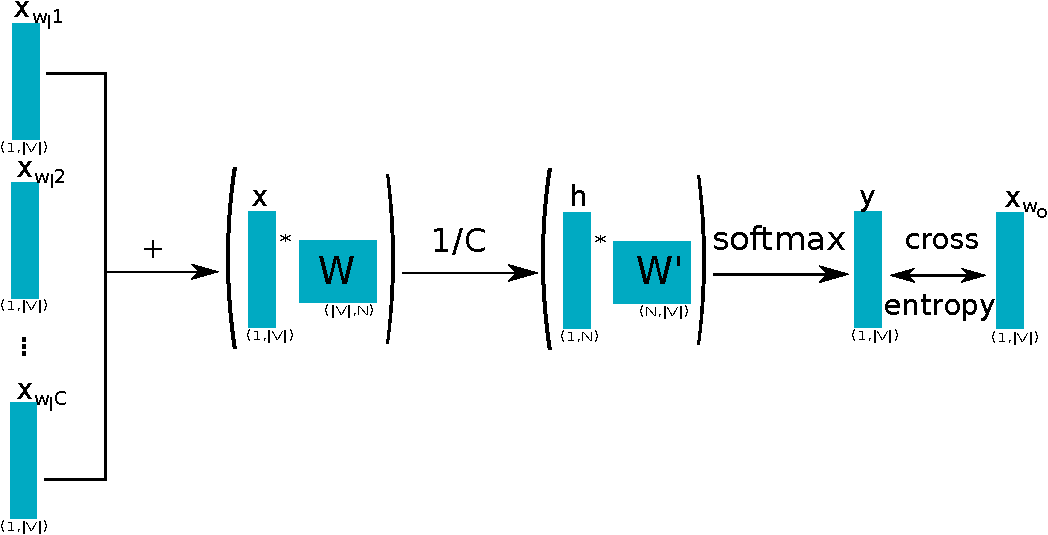
\includegraphics[scale=0.65]{cbow.pdf}
\end{frame}

\begin{frame}[fragile]{CBOW: modelo (ii)}
\begin{equation}\label{eq:13}
{\color{blue!89}x = x_{\wo_{I_{1}}} + \dots + x_{\wo_{I_{C}}}}
\end{equation}
\begin{equation}\label{eq:14}
{\color{blue!89}h = \frac{1}{C}(v_{\wo_{I_{1}}} + \dots + v_{\wo_{I_{C}}}) }
\end{equation}
\begin{equation}\label{eq:15}
u_j = \sum_{s=1}^{N}w^{\prime}_{sj} h_{s}
\end{equation}
\begin{equation}\label{eq:16}
y_j = p(\wo_{j}|\wo_{I_{1}},\dots, \wo_{I_{C}}) =  \frac{\exp(v^{\prime}_{\wo_{j}} .^{T} h)}{\sum_{j^{\prime}=1}^{|V|} \exp(v^{\prime}_{\wo_{{j^\prime}}} .^{T} h)} 
\end{equation}
\begin{equation}\label{eq:17}
E = - u_{j^{*}} + \log (\sum_{j^{\prime}=1}^{|V|} \exp (u_{j^{\prime}}))
\end{equation}
\end{frame}


\begin{frame}[fragile]{CBOW: atualização}

\begin{equation}\label{eq:18}
{v^{\prime}_{\wo_{j}}}^{(new)} = {v^{\prime}_{\wo_{j}}}^{(old)} - \eta \, e_{j} \, h
\end{equation}

\vspace{0.3cm}

\begin{equation}\label{eq:19}
{v_{\wo_{I_{c}}}}^{(new)} = {v_{\wo_{I_{c}}}}^{(old)} - \frac{1}{C} \, \eta \, x EH^{T}_{(k_{I_{c}},.)} 
\end{equation}

\vspace{0.3cm}

para $c = 1, \dots, C$. Onde $k_{I_{1}}, \dots, k_{I_{C}}$ são os índices de $\wo_{I_{1}},\dots, \wo_{I_{C}}$ respectivamente.
\end{frame}

\begin{frame}[fragile]{Skip-Gram}
\begin{center}
Skip-gram é o "contrário" do CBOW.
\end{center}

\vspace{0.3cm}

\textbf{Com esse modelo vamos tentar prever o contexto dado a palavra de centro.}\\

\vspace{0.3cm}

Observação $\Rightarrow$ $(\wo_{I},[\wo_{O_{1}},\dots, \wo_{O_{C}}])$\\

\vspace{0.1cm}

{\color{white!89}Observação } $\Rightarrow$ (cantor, [com, o, dessa, banda])
\end{frame}

\begin{frame}[fragile]{Skip-Gram: modelo (i)}
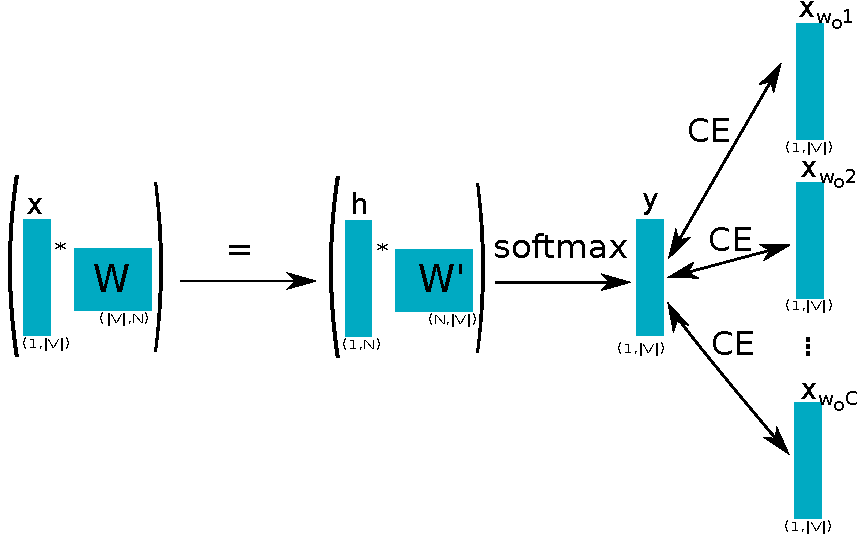
\includegraphics[scale=0.65]{skip-gram.pdf}
\end{frame}

\begin{frame}[fragile]{Skip-Gram: modelo (ii)}
As definições de $x$, $h$, $u$, e $y$ são as mesmas que em (\ref{eq:1}), (\ref{eq:2}) e (\ref{eq:3}). Nesse modelo queremos minimizar a soma da entropia cruzada que é o mesmo que maximizar $p(\wo_{o_{1}}, \dots, \wo_{o_{C}}\;|\;\wo_I)$:
 
\begin{align*}
E & = \sum_{c=1}^{C}(-\sum_{s=1}^{V} {\wo_{o_{c}}}_s \log(y_s)) \\
& = - \sum_{c=1}^{C} \log(y_{j^{*}_{c}})\\
& = - \log(\prod_{c=1}^{C}y_{j^{*}_{c}})\\
& = - \log(\prod_{c=1}^{C}p(\wo_{o_{c}}\;|\;\wo_I))\\
& = - \log p(\wo_{o_{1}}, \dots, \wo_{o_{C}}\;|\;\wo_I)\\
\end{align*}
\end{frame}
\begin{frame}[fragile]{Skip-Gram: modelo (iii)}
Simplificando a equação de erro:
\begin{equation}\label{eq:20}
E = - \sum_{c=1}^{C} u_{j^{*}_{c}} + C \log (\sum_{j^{\prime}=1}^{V} \exp (u_{j^{\prime}}))
\end{equation}
\end{frame}

\begin{frame}[fragile]{Skip-Gram: atualização}
\begin{equation}\label{eq:21}
{v^{\prime}_{\wo_{j}}}^{(new)} = {v^{\prime}_{\wo_{j}}}^{(old)} - \eta \, e_{j} \, v_{\wo_{I}}
\end{equation}

\vspace{0.3cm}

\begin{equation}\label{eq:22}
{v_{\wo_{I}}}^{(new)} = {v_{\wo_{I}}}^{(old)} - \eta \, x EH^{T}_{(k_{I},.)} 
\end{equation}

\vspace{0.3cm}

Onde $e = (Cy - \sum_{c=1}^{C}x_{\wo_{c}})$  e $EH = e {(W^{\prime})}^{T}$.
\end{frame}


\begin{frame}[fragile]{Otimização}
\[
y_j = \frac{\exp(u_j)}{\sum_{j^{\prime}=1}^{|V|} \exp(u_{j^{\prime}})} 
\]
\begin{center}
\textbf{Muito custoso se for fazer isso para cada instância de treinamento}
\end{center}
\vspace{0.3cm}

\begin{itemize}
\item Amostragem negativa
\vspace{0.2cm}
\item Softmax hierárquico
\end{itemize}


\end{frame}

\begin{frame}[fragile]{Otimização}
Vamos nos concentrar no modelo Skip-gram. 

\vspace{0.2cm}

\textbf{Note}: podemos implementar esse modelo de modo a prever apenas uma palavra de contexto:\\

\[
(cantor, [com, o, dessa, banda])
\]
\[
(cantor,com), (cantor,o), (cantor,dessa), (cantor,banda)
\]

\textbf{Note}
\begin{itemize}
\item Skip-gram $\Rightarrow h = v_{\wo_I}$ 
\vspace{0.1cm}
\item CBOW $\Rightarrow h = \frac{1}{C}\sum_{c=1}^{C}v_{\wo_{I_{c}}}$ 
\end{itemize}

\end{frame}



\begin{frame}[fragile]{Amostragem negativa}
Vamos manter $x$, $W$ e $W^{\prime}$ e $h$ como antes. Para calcular a função erro vamos usar uma distribuição $P_{n}(\wo)$ sobre as palavras do corpus. Exemplo:\\
\[
P_{n}(\wo) = \frac{U(\wo)^{\frac{3}{4}}}{Z}
\]
\vspace{0.1cm}
Usando $P_{n}(\wo)$ vamos amostrar $\wo_{i_{1}}, \dots , \wo_{i_{K}}$; garantindo que $\wo_{o}$ não está entre elas. 
\end{frame}
\begin{frame}[fragile]{Amostragem negativa}
\[
{\color{blue!89}(\wo_{I},\wo_{O})}
\]
\begin{center}
{\color{blue!89}Exemplo positivo}
\end{center}

\[
{\color{red!89}(\wo_{I},\wo_{i_{1}}), \dots, (\wo_{I},\wo_{i_{K}})}
\]
\begin{center}
{\color{red!89}Exemplos negativos}
\end{center}


\end{frame}
\begin{frame}[fragile]{Amostragem negativa: o modelo (i)}
\[
p(D=1 \;|\; \wo_I,\wo) = \sigma(v_{\wo}^{\prime} \; .^{T} \;h)
\]
\begin{center}
probabilidade do par $(\wo_{I},\wo)$ ocorrer no corpus 
\end{center}
\[
p(D=0 \;|\; \wo_I,\wo)
\]
\begin{center}
probabilidade do par $(\wo_{I},\wo)$ não ocorrer no corpus 
\end{center}
\vspace{0.3cm}
O objetivo de treinamento agora é maximizar as probabilidades  
\[
{\color{blue!89}p(D=1 \;|\; \wo_I,\wo_{O}),\; p(D=0 \;|\; \wo_I,\wo_{i_{1}}), \dots , \; p(D=0 \;|\; \wo_I,\wo_{i_{K}})}
\]
\end{frame}

\begin{frame}[fragile]{Amostragem negativa: o modelo (ii)}
Assim, vamos minimizar a seguinte função erro:
\begin{align*}
E & = -\log (p(D=1 \;|\; \wo_I,\wo_{O}) \, .\, \prod_{s=1}^{K} p(D=0 \;|\; \wo_I,\wo_{i_{s}})) \\
& = - (\log p(D=1 \;|\; \wo_I,\wo_{O}) + \log(\prod_{s=1}^{K} p(D=0 \;|\; \wo_I,\wo_{i_{s}})))\\
& = - (\log p(D=1 \;|\; \wo_I,\wo_{O}) + \sum_{s=1}^{K}\log(p(D=0 \;|\; \wo_I,\wo_{i_{s}})))\\
& = - \log \sigma(v_{\wo_O}^{\prime} \; .^{T} \; h) - \sum_{s=1}^{K}\log(\sigma(- v_{\wo_{i_{s}}}^{\prime} \; .^{T} \; h))\\
\end{align*}
\end{frame}

\begin{frame}[fragile]{Amostragem negativa: atualização}

\begin{equation}\label{eq:23}
{v^{\prime}_{\wo_{O}}}^{(new)} = {v^{\prime}_{\wo_{O}}}^{(old)} - \eta \, (\sigma( v_{\wo_{O}}^{\prime} \; .^{T} \; h) -1) \, h
\end{equation}

\begin{equation}\label{eq:24}
{v^{\prime}_{\wo_{i_{s}}}}^{(new)} = {v^{\prime}_{\wo_{i_{s}}}}^{(old)} - \eta \, \#(i_{s})  \, \sigma(v_{\wo_{i_{s}}}^{\prime} \; .^{T} \; h) \, h
\end{equation}

\begin{equation}\label{eq:25}
W^{(new)} = W^{(old)} - \eta \, x EH^{T}
\end{equation}

\vspace{0.3cm}
Onde 
\[
EH = (\sigma(v_{\wo_{O}}^{\prime} \; .^{T} \; h) -1) \, v_{\wo_{O}}^{\prime} + \sum_{s=1}^{K}\sigma(v_{\wo_{i_{s}}}^{\prime} \; .^{T} \; h)v_{\wo_{i_{s}}}^{\prime}
\]
e $\#(i_{s})$ é a contagem de $i_{s}$.
\end{frame}


\begin{frame}[fragile]{Softmax hierárquico: motivação}
\begin{displayquote}
\textit{The basic idea is to form a hierarchical description of a word as a sequence of $O(\log |V|)$ decisions, and to learn to take these probabilistic decisions instead of directly predicting each word's probality.}(Morin and Bengio 2005, p.247)
\end{displayquote}


\end{frame}

\begin{frame}[fragile]{Softmax hierárquico: árvore de Huffman}
[(de, $24480774$), (repreendeu, $401$), (eróticas, $424$), (adesões, $400$)] 

\begin{center}
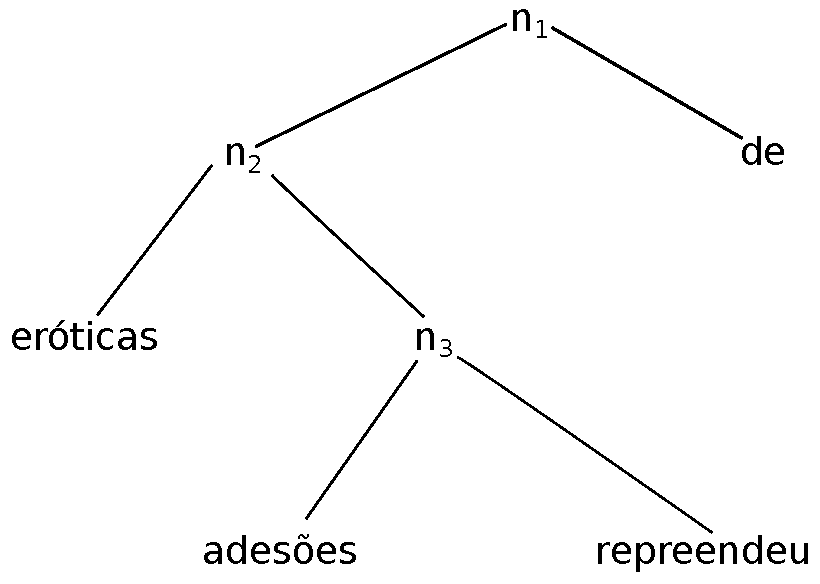
\includegraphics[scale=0.5]{tree.pdf}
\end{center}
$\{$ de:$1$, eróticas: $00$, adesões:$010$, repreendeu:$011 \}$. 

\end{frame}

\begin{frame}[fragile]{Softmax hierárquico: notação}
\begin{itemize}
\item Dado um vocabulário $V$, temos $|V|-1$ vértices que não são folhas (\textit{nós internos}). 
\item O caminho da raiz até a folha vai ser usado para estimar a probabilidade da palavra representada pela folha.
\item  Dado a palavra $\wo$, $L(\wo)$ é o comprimento do caminho da raiz até $\wo$  e $n(\wo,1), \dots, n(\wo, L(\wo)-1)$ são todos os nós internos no caminho da raiz até $\wo$.\
\item $H(\wo)_j$ vai denotar o $j$-ésimo número de código de $\wo$. $1$ vai codificar esquerda e $-1$ vai codificar direita.
\end{itemize}
$\{$ de:$-1$, eróticas: $11$, adesões:$1-11$, repreendeu:$1-1-1 \}$. 
\end{frame}

\begin{frame}[fragile]{Softmax hierárquico: o modelo}

Dado uma observação $(\wo_I,\wo_O)$ os cálculos de $x$ e $h$ vão ser os mesmos; $W$ ainda guarda os \textit{input vectors}. No lugar dos \textit{output vectors} temos: 

\vspace{0.2cm}

\[
v^{\prime}_{n(\wo,j)} 
\]

\vspace{0.2cm}

para cada nó interno $n(\wo,j)$.

\end{frame}

\begin{frame}[fragile]{Softmax hierárquico}
 Dado $\wo_I$, cada nó interno tem uma probabilidade associada de ir para a esquerda ou para a direita:
\begin{equation}\label{eq:26}
p(n(\wo,j), esquerda) = \sigma(v^{\prime}_{n(\wo,j)} \; .^{T} \; h)
\end{equation}
\begin{equation}\label{eq:27}
p(n(\wo,j), direita) = \sigma(- v^{\prime}_{n(\wo,j)} \; .^{T} \; h)
\end{equation}
Desse modo, temos que dado a ocorrência de $\wo_I$ a probabilidade da palavra $\wo$ ser $\wo_O$ é:
\begin{equation}\label{eq:28}
p(\wo = \wo_O\; |\; \wo_I) = \prod_{j=1}^{L(\wo_{O})-1} \sigma(H(\wo_O)_j . v^{\prime}_{n(\wo_{O},j)} \; .^{T} \; h)
\end{equation}
\end{frame}

\begin{frame}[fragile]{Softmax hierárquico}
Como queremos maximizar $p(\wo = \wo_O\; |\; \wo_I) $ a função de erro que queremos minimizar é 

\begin{equation}\label{eq:29}
E = - \log p(\wo = \wo_O\; |\; \wo_I)
\end{equation}

\end{frame}

\begin{frame}[fragile]{Softmax hierárquico: atualização}
\begin{equation}\label{eq:30}
{v^{\prime}_{n(\wo_{O},j)}}^{(new)} = {v^{\prime}_{n(\wo_{O},j)}}^{(old)} - \eta \, (\sigma(  v^{\prime}_{n(\wo_{O},j)} \; .^{T} \; h) -t_{j}) \,h
\end{equation}

\vspace{0.1cm}

\begin{equation}\label{eq:31}
W^{(new)} = W^{(old)} - \eta \, x EH^{T}
\end{equation}

\vspace{0.1cm}

\vspace{0.3cm}
Onde,
\[
t_{j}=
\begin{cases}
1, \text{ se } H(\wo)_{j} =1\\
0, \text{ se } H(\wo)_{j} =-1
\end{cases}
\]

\vspace{0.2cm}

\[
EH = \sum_{j=1}^{L(\wo_O) -1} (\sigma(v_{n(\wo,j)}^{\prime} \; .^{T} \; h) - t_j) {v_{n(\wo,j)}^{\prime}}
\]
\end{frame}



\begin{frame}[fragile]{Exemplo de aplicação: NER}
\textbf{NER: named entity recognition} (extração de entidades nomeadas).
Dada uma sentença queremos saber quais entidades ocorrem nela, assim temos de um lado sentenças e de outro categorias (pessoa, localização, organização).

\vspace{0.1cm}

\textbf{Modelo de janela :} observações do tipo 

\[
([\wo_{t-m}, \dots, \wo_{t}, \dots, \wo_{t+m}],c)
\]
\begin{center}
("A comissão europeia discorda do tratado proposto", ORG)
\end{center}
\end{frame}

\begin{frame}[fragile]{Exemplo de aplicação: NER}
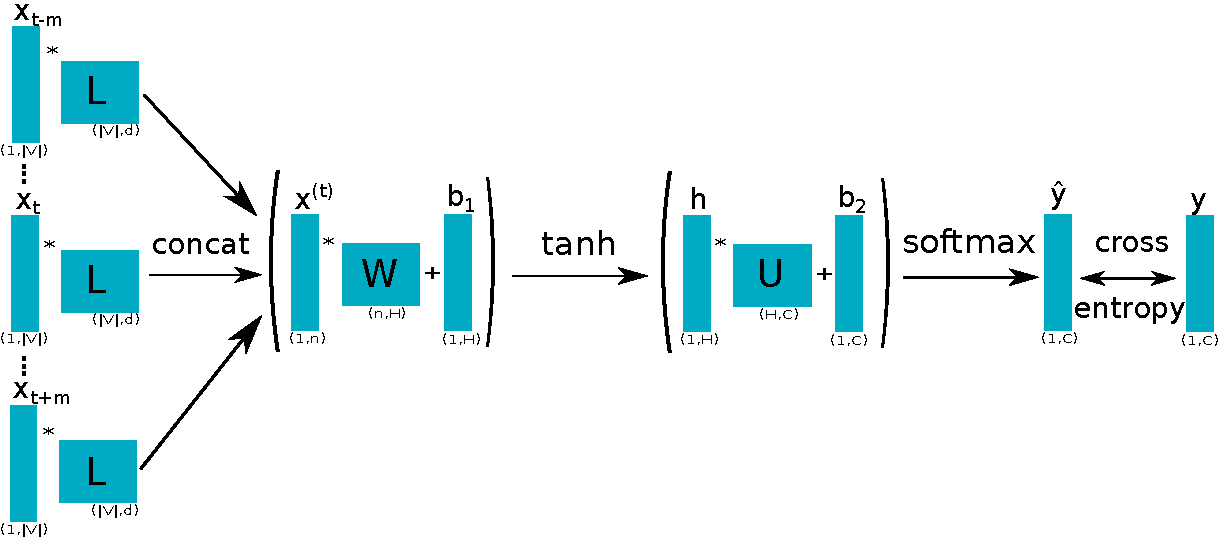
\includegraphics[scale=0.57]{ner.pdf}
\end{frame}

\begin{frame}[fragile]{Como avaliar o modelo?}
\begin{itemize}
\item \textbf{avaliação intrínseca :} avaliação rápida feita numa tarefa intermediaria: e.g., predição de analogias semânticas.
\vspace{0.3cm}
\item \textbf{avaliação extrínseca :} avaliação feita numa tarefa real de NLP: e.g., NER.
\end{itemize}
\end{frame}

\begin{frame}[fragile]{Como avaliar o modelo? Avaliação intrínseca}
\begin{center}
\textbf{$\wo_{a}$ está para $\wo_{b}$ assim como $\wo_{c}$ está para $\_$}\\
rapaz moça irmãos irmãs\\
trabalhou trabalham gerar geram\\
homem mulher rei rainha
\end{center}
\[
\wo_{a}:\wo_{b} \rightarrow \wo_{c}: ?
\]
\begin{equation}\label{eq:32}
\wo_{d} = arg max_{x} \; \frac{(b-a +c).^{T}x}{||b-a +c||}
\end{equation}

\begin{equation}\label{eq:33}
\wo_{d} = arg max_{x}  \; b.^{T}x -a.^{T}x +c.^{T}x
\end{equation}
\begin{center}
\textbf{ Qual a palavra cuja representação é similar a $\wo_{b}$ e $\wo_{c}$ e dissimilar de $\wo_{a}$?}
\end{center}

\end{frame}

\begin{frame}[fragile]{Avaliação intrínseca}
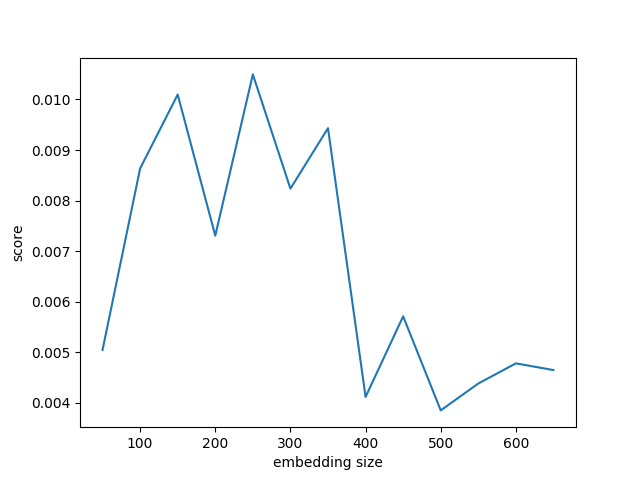
\includegraphics[scale=0.69]{emb_size}
\end{frame}

\begin{frame}[fragile]{Implementação: https://github.com/felipessalvatore/Word2vec-pt}
\begin{center}
\small{Corpus em português}
\end{center}
\small{
\begin{figure}
\begin{center}
\begin{tabular}{|c|c|c|}
\hline
\cellcolor{blue!40}Categoria & \cellcolor{blue!40}Word2vec-pt & \cellcolor{blue!40}Gensim  \\ \hline
\cellcolor{blue!10}capital-common-countries & \cellcolor{green!20}(15/306) &  \cellcolor{green!20}(8/90) \\ \hline
\cellcolor{blue!10}capital-world &  \cellcolor{green!20}(7/1155) & \cellcolor{green!20} (4/173) \\ \hline
\cellcolor{blue!10}curency & \cellcolor{green!20} (0/106) &  \cellcolor{green!20}(0/54) \\ \hline
\cellcolor{blue!10}city-in-state & \cellcolor{green!20} (1/1171) &  \cellcolor{green!20}(1/208) \\ \hline
\cellcolor{blue!10}family &  \cellcolor{red!20}(41/342) & \cellcolor{red!20}(132/306) \\ \hline
\cellcolor{blue!10}gram1-adjective-to-adverb &  \cellcolor{red!20}(1/552) & \cellcolor{red!20}(5/380)  \\ \hline
\cellcolor{blue!10}gram2-opposite &  \cellcolor{red!20}(0/182) &\cellcolor{red!20}(3/90) \\ \hline
\cellcolor{blue!10}gram3-comparative &  \cellcolor{red!20}(5/30) & \cellcolor{red!20}(12/30) \\ \hline
\cellcolor{blue!10}gram4-superlative &  \cellcolor{red!20}(3/20) & \cellcolor{red!20}(4/6) \\ \hline
\cellcolor{blue!10}gram5-present-participle & \cellcolor{red!20} (0/702) & \cellcolor{red!20}(61/462) \\ \hline
\cellcolor{blue!10}gram6-nationality-adjective & \cellcolor{red!20}(0/412) & \cellcolor{red!20}(37/739) \\ \hline
\cellcolor{blue!10}gram7-past-tense &  \cellcolor{red!20}(8/1056) & \cellcolor{red!20}(124/506) \\ \hline
\cellcolor{blue!10}gram8-plural & \cellcolor{red!20} (1/992) &\cellcolor{red!20} (25/380) \\ \hline
\cellcolor{blue!10}gram9-plural-verbs &  \cellcolor{red!20}(9/552) & \cellcolor{red!20}(29/306)
\end{tabular}
\end{center}
\end{figure}
}
\end{frame}

\begin{frame}[fragile]{Implementação: https://github.com/felipessalvatore/Word2vec-pt}

% EUUUUUUUU
% family: 13.5% (46/342)
% gram1-adjective-to-adverb: 0.6% (6/930)
% gram2-opposite: 0.0% (0/506)
% gram3-comparative: 2.7% (36/1332)
% gram4-superlative: 0.7% (5/756)

% gram5-present-participle: 1.4% (15/1056)
% gram7-past-tense: 1.5% (22/1482)
% gram8-plural: 1.4% (17/1190)
% gram9-plural-verbs: 1.0% (8/812)
\begin{center}
\small{Corpus em inglês}
\end{center}

\small{
\begin{figure}
\begin{center}
\begin{tabular}{|c|c|c|}
\hline
\cellcolor{blue!40}Categoria & \cellcolor{blue!40}Word2vec-pt & \cellcolor{blue!40}Gensim  \\ \hline
\cellcolor{blue!10}family &  \cellcolor{green!20}(46/342) & \cellcolor{green!20}(1/306) \\ \hline
\cellcolor{blue!10}gram1-adjective-to-adverb &  \cellcolor{green!20}(6/930) & \cellcolor{green!20}(0/756)  \\ \hline
\cellcolor{blue!10}gram2-opposite &  \cellcolor{green!20}(0/506) &\cellcolor{green!20}(0/306) \\ \hline
\cellcolor{blue!10}gram3-comparative &  \cellcolor{green!20}(36/1332) & \cellcolor{green!20}(0/1260)\\ \hline
\cellcolor{blue!10}gram4-superlative &  \cellcolor{green!20}(5/756) & \cellcolor{green!20}(0/506) \\ \hline
\cellcolor{blue!10}gram5-present-participle & \cellcolor{green!20} (15/1056) & \cellcolor{green!20}(0/992) \\ \hline
\cellcolor{blue!10}gram7-past-tense &  \cellcolor{green!20}(22/1482) & \cellcolor{green!20}(0/1332) \\ \hline
\cellcolor{blue!10}gram8-plural & \cellcolor{green!20} (17/1190) &\cellcolor{green!20} (0/992) \\ \hline
\cellcolor{blue!10}gram9-plural-verbs &  \cellcolor{green!20}(8/812) & \cellcolor{green!20}(0/650)
\end{tabular}
\end{center}
\end{figure}
}
\end{frame}


\begin{frame}[fragile]{Bibliografia}

\begin{itemize}
\item Mikolov, T., Chen, K., Corrado, G., and Dean, J. (2013). Efficient estimation of word representation in vector space. \textit{arXiv preprint arXiv:1301.3781}.
\item Mikolov, T., Sutskever, I., Chen, K., Corrado, G., and Dean, J. (2013). Distributed representations of words and phrases and their compositionality. In \textit{Advances in Neural Information Processing Systems}, pages 3111-3119.
\item Morin, F., Bengio, Y. (2005). Hierarchical probabilistic neural network language model. In \textit{AISTATS}, pages 246-252.
\item Rong, X. (2016). Word2vec Parameter Learning Explained. \textit{arXiv preprint arXiv:1411.2738}.


\end{itemize}

\end{frame}





\end{document}
